\section{Critique}
\label{sec:critique}

\begin{frame}{Verification and Validation}
  \begin{itemize}
    \item No spatial convergence results.
    \item Single verification benchmark presented: \gls{iaea} 3D \gls{pwr}.
    \item Pebble bed reactor results not verified.
    \item $\lambda$ and $\| \residual(\vx^m) \|$ not related so convergence of
      $\lambda$ cannot be inferred.
  \end{itemize}
\end{frame}

\begin{frame}{Critical Boron Concentration Search}
  \begin{itemize}
    \item Typically for \glspl{pwr}, the critical boron concentration is
      desired such that $\lambda = 1.0$.
    \item Current algorithm is linked to the \gls{pi} method.
    \item May be extendable to the \gls{jfnk} method or may be too inefficient
      to undo any efficiency improvements.
  \end{itemize}
\end{frame}

\begin{frame}{\glsentrylong{cmfd} Formulation}
  \begin{itemize}
    \item \citeauthor{qe2paper} solve for \gls{nem} coefficients directly.
    \item Instead, a $\dtilde$ can be calculated to correct the finite
      difference equations \cite{smith_nonlinear,palmtagThesis}.
    \item Solution vector is reduced $10 \times N \times G \rightarrow N \times G$.
    \item Would be compatible with existing codes \cite{casmo4,simulate3,mpact}.
    \item May pose additional challenges compared to \gls{pi} method.
  \end{itemize}
  \begin{multline}
    \label{eq:dtilde}
    \current_{g,u}(u) = 
      -2 \left( \frac{h_{\ell+1}}{\overline{D}_{g,\ell+1}} + 
        \frac{h_{\ell}}{\overline{D}_{g,\ell}} \right)^{-1}
        \left( \overline{\phi}_{g,u,\ell+1} -
        \overline{\phi}_{g,u,\ell} \right) +  \\
      \dtilde_{g,u} \left( \overline{\phi}_{g,u,\ell+1} +
        \overline{\phi}_{g,u,\ell} \right)
  \end{multline}
\end{frame}

\begin{frame}{Ragged Core}
  \begin{itemize}
    \item After performing local elimination, 18\% of the solution variables are
      still unnecessary.
    \item This may bias results and penalize the \gls{pi} method
      \cite{gehinThesis}.
  \end{itemize}
  \begin{figure}
    \centering
    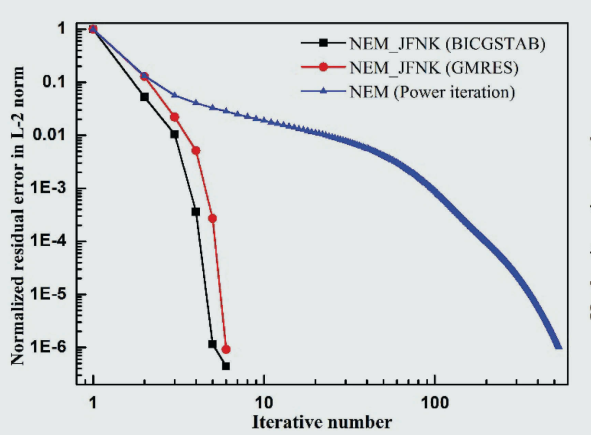
\includegraphics{./figs/iaea3d_convergence.png}
  \end{figure}
\end{frame}

\begin{frame}{\glsentrylong{ws}}
  \begin{itemize}
    \item \gls{ws} can reduce \gls{pi} method runtime by a factor of three or
      more.
    \item \citeauthor{qe2paper} do not compare the \gls{jfnk} method to a
      \gls{pi} method with the \gls{ws}.
    \item \gls{ws} could invalidate some of the results.
    \item \gls{jfnk} may still be preferable to \gls{pi}+\gls{ws} \cite{jfnk_wielandt}.
    \item \gls{ws} would also be useful for a \gls{pi} preconditioner.
  \end{itemize}
\end{frame}
